\chapter{Implementation}\chaplabel{4}

This chapter provides a detailed explanation of how to detect roller shutters using the PyTorch framework and the YOLOv5-v6.0 algorithm.

\section{Process Handover and Overview}

This bachelor thesis is mainly focused on detecting the status of roller shutters, while the localization of window position has been addressed in another bachelor thesis titled "Building Management: AI Mapping Image to Construction Plan" by Tao Liu. For more information regarding window localization, please refer to the aforementioned thesis. This section will also give a brief introduction of the handover process.

\begin{figure}[h]
  \centering
  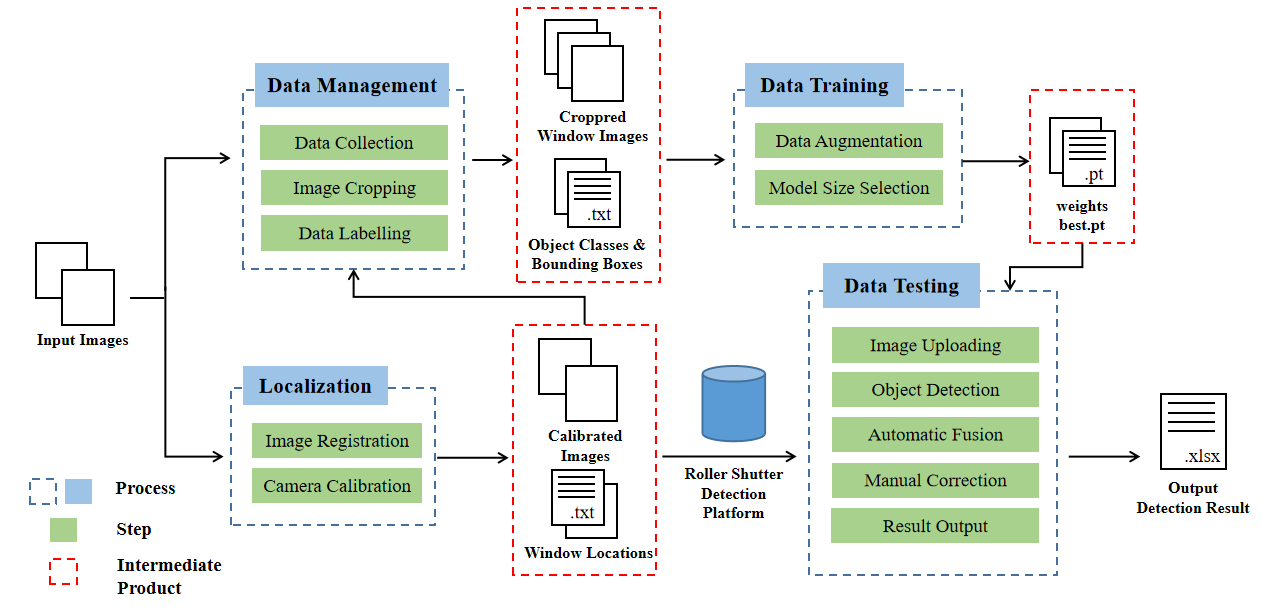
\includegraphics[width=1\textwidth]{Figures/process overview.png}
  \caption{An Overview of the Work Flow}
  \label{fig:15}  
\end{figure}

As shown in Figure \ref{fig:15}, the inputs for the entire process are building images captured by pre-set cameras on the THL campus. Tao's work involves processing these raw images into calibrated images and outputting window locations as coordinates in a text file. My work involves taking these calibrated images and window locations as inputs, and outputting the detection results, including the roller shutter status and the Degree of Closure (DoC) of each window, in an Excel file.

To enable an end-to-end process, a roller shutter detection platform is set up using the Qt Designer tool in Python, and the YOLO model is loaded for detection. Prior to loading the model, data management and data training are two critical modules for obtaining the necessary weights, which are essential for the detection model to function properly. Both raw input images and calibrated images are involved in the data collection process. These images are then manually cropped or cropped according to coordinates into separated window images for the labeling process followed. The following sections will provide a detailed explanation of each process module.

\section{Data Management}

Data Management involves three steps, which are data collection, image cropping and data labeling before adding to the training data set.

\subsection{Image Acquisition and Preprocessing}

\subsection{Labeling Strategies}


\section{Data Training}

After labeling, a text file recording the object classes and bounding boxes coordinates is generated for each cropped images. Before the training started, the model size of YOLO needs to be decided and customized data augmentation would also be an option.

\subsection{Data augmentation}

To improve the performance of detection model in different lighting conditions and robustness against occlusion. Two data augmentation methods are used, which are cutout and adjusting brightness. Cutout is the process to randomly dig out a specified number of small squares of a specified size from the image. This process can improve the robustness of the model against mild occlusions. 

\subsection{Model Selection}

\section{Data Testing and Detection Platform}

After the weights are obtained from training process, we can load this model to test its performance. In this bachelor thesis, a roller shutter detection platform is designed as the final product and evaluation tools. The following subsection will introduce its features and functions. Figure \ref{fig:16} below gives an overview of the activity flow.

\begin{figure}[h]
  \centering
  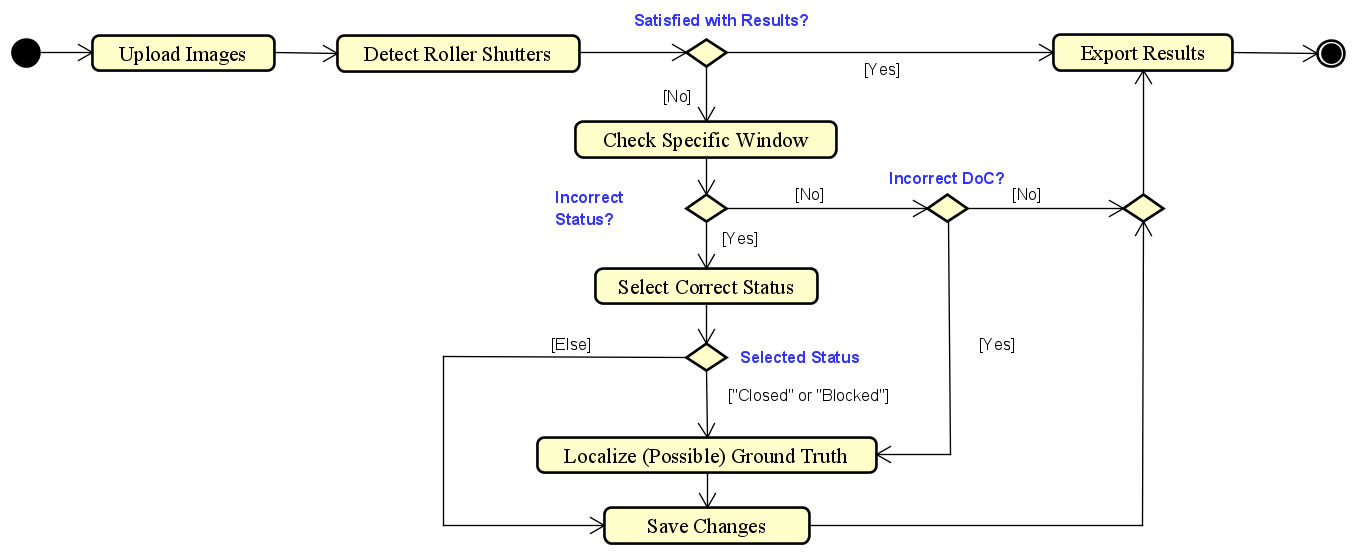
\includegraphics[width=1\textwidth]{Figures/Activity Diagram.png}
  \caption{An Overview of the Work Flow}
  \label{fig:16}  
\end{figure}

\subsection{Image Upload}


\textbf{Check Image Taken Time}

\textbf{Cropping and Warping}

\subsection{Roller Shutter Detection}

\textbf{Iterate through cropped images}

\textbf{Detect roller shutter and glass}

\textbf{Draw bounding boxes}

\subsection{Automatic Fusion}



\textbf{Fusion Logic}

\textbf{Obtain final DoC}

\subsection{Manual Correction}

\textbf{Change Status and DoC}

\subsection{Report Export}



